\documentclass[tikz,svgnames]{standalone}

\begin{document}
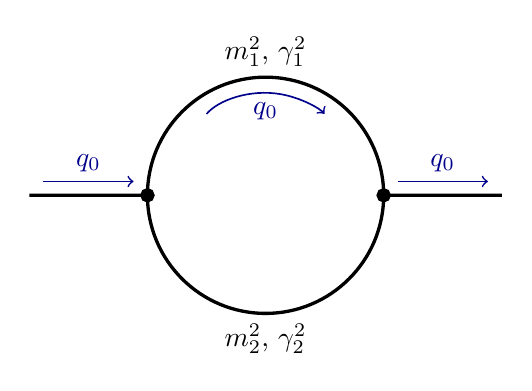
\begin{tikzpicture}[very thick,q0/.style={->,DarkBlue,semithick,yshift=5pt,shorten >=5pt,shorten <=5pt}]

  % Loop
  \def\radius{1.5}
  \draw (0,0) circle (\radius);
  \node[above] (1) at (0,\radius) {$m_1^2$, $\gamma_1^2$};
  \node[below] (2) at (0,-\radius) {$m_2^2$, $\gamma_2^2$};
  \draw[q0] (140:0.75*\radius) arc (140:40:0.75*\radius) node[midway,below] {$q_0$};

  % External lines
  \filldraw
  (-2*\radius,0) -- (-\radius,0) circle (2pt)
  (\radius,0) circle (2pt) -- (2*\radius,0);
  \draw[q0] (-2*\radius,0) -- (-\radius,0) node[midway,above] {$q_0$};
  \draw[q0] (\radius,0) -- (2*\radius,0) node[midway,above] {$q_0$};


\end{tikzpicture}
\end{document}